%!TEX root = ../compendium.tex

\Lab{\LabWeekONE}

\subsubsection{Mål}
\begin{itemize}[nosep]
\item Kunna kombinera principerna sekvens, alternativ, repetition, och abstraktion i skapandet av egna program om minst 20 rader kod.
\item Kunna förklara vad ett program gör i termer av sekvens, alternativ, repetition, och abstraktion.
\item Kunna formatera egna program så att de blir lätta att läsa och förstå.
\item Kunna genomföra upprepade varv i cykeln \emph{editera-exekvera-felsöka/förbättra} för att succesivt bygga upp allt mer utvecklade program. 
\item Kunna identifiera liknande satser och utifrån dessa skapa återanvändbara abstraktioner.
\end{itemize}

\subsubsection{Förberedelser}
\begin{itemize}[nosep]
\item Gör övning {\tt \ExeWeekONE} i kapitel \ref{exe:W01}.
\item Läs igenom ''Kojo - An Introduction'' (25 sidor) som du kan ladda ner i pdf  här: \href{http://www.kogics.net/kojo-ebooks}{http://www.kogics.net/kojo-ebooks}
\item Du behöver en dator med Kojo installerad, se appendix \ref{appendix:kojo}.
\end{itemize}

\subsection{Obligatoriska uppgifter}


\Task \textit{Sekvens}. 

\Subtask Starta Kojo. Om du inte redan har svenska menyer: välj svenska i språkmenyn och starta om Kojo.  Skriv in nedan program och tryck på den \emph{gröna} play-knappen. Du hittar en lista med några fler funktioner på svenska och engelska i appendix \ref{appendix:kojo}.

\begin{Code}
sudda

fram; höger
fram; vänster
\end{Code}


\Subtask Prova att ändra på ordningen mellan satserna och använd den \emph{gula} play-knappen  (programspårning) för att studera vad som händer. Klicka på satser i ditt program och på rutor i programspårningen och se vad som händer.

\Subtask Prova satser i sekvens på flera rader, respektive på samma rad med semikolon emellan. Hur vill du gruppera dina satser så att de lätta för en människa att läsa?

\Subtask\Pen Vad händer om du inte börjar programmet med \code{sudda} och kör det upprepade gånger? Varför är det bra börja programmet med \code{sudda}? 

\Subtask Rita en kvadrat som i bilden nedan.

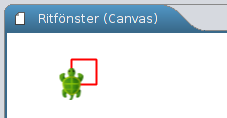
\includegraphics{../img/kojo/kvadrat}

\Subtask Ge \code{fram} en parameter så att kvadraten blir större.  Prova att med höger-klick i ritfönstret visa rutnät och koordinataxlar.




\Subtask\Checkpoint Rita en triangel genom att ge lämplig vinkel som parameter till det kommando som orsakar vridningen av sköldpaddan. Vridningen anges i grader och ett helt varv motsvarar 360 grader.



\Task \textit{Repetition}. 

\Subtask Rita en kvadrat igen, men nu med hjälp av proceduren \code+upprepa(n){ ??? }+ där du ersätter n med antalet repetitioner och ??? med de satser som ska repeteras. 

\Subtask Anropa proceduren \code{sakta(???)} med lämplig parameter och gör så att sköldpaddan går totalt 20 varv i kvadraten på ungefär 2 sekunder. \emph{Tips:} Du kan köra ditt program med \emph{Ctrl+Enter} i stället för att trycka på den gröna play-knappen. Anropa \code{sakta} i början av ditt program men \emph{efter} sudda. (Vad händer om du anropar \code{sakta} före \code{sudda}?)


\Subtask Om du anropar \code{sakta(0)}, hur många kvadratvarv hinner sköldpaddan rita på en sekund? Använd nedan program för att ta reda på ungefärligt antal varv per sekund.
\begin{Code}
sudda; sakta(0)
val t1 = System.currentTimeMillis
upprepa(800*4){fram;höger}
val t2 = System.currentTimeMillis
println("Det tog " + (t2 - t1) + " millisekunder")
\end{Code} 



\Subtask Rita en kvadrat igen, men nu med hjälp av en \code{while}-sats och en loop-variabel.

\begin{Code}
var i = 0
while (???) {fram; höger; i = ???}
\end{Code} 

\Subtask Rita en kvadrat igen, men nu med hjälp av en \code{for}-sats.

\begin{Code}
for (i <- 1 to ???) {???}
\end{Code} 

\Subtask Rita en kvadrat igen, men nu med hjälp av \code{foreach}.

\begin{Code}
(1 to ???).foreach{i => ???}
\end{Code} 


\Subtask\Pen Vad är fördelar och nackdelar med de olika sätten att loopa: \code{upprepa}, \code{while} respektive \code{for}.

\Task \textit{Abstraktion}. 

\Subtask Använd proceduren \code{kvadrat} nedan och proceduren \code{hoppa(???)} för att rita en stapel med 10 kvadrater enligt bilden.

\begin{Code}
def kvadrat = upprepa(4){fram; höger}
\end{Code}

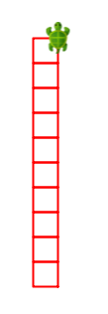
\includegraphics[scale=0.5]{../img/kojo/square-column}


\Subtask Rita flera kvadrater som i bilden nedan.


\includegraphics{../img/kojo/square-param}



\Task \textit{Alternativ}.

\Task \textit{Tidmätning}. Hur snabb är din dator?

\Subtask \label{task:timer} Skriv in koden nedan i Kojos editor och kör med den gröna play-knappen. Hur långt tid tar det för din dator att räkna till 4.4 miljarder?

\begin{Code}
object timer {
  def now: Long = System.currentTimeMillis
  var saved: Long = now
  def elapsedMillis: Long = now - saved
  def elapsedSeconds: Double = elapsedMillis / 1000.0
  def reset: Unit = { saved = now }
}

// HUVUDPROGRAM:
timer.reset
var i = 0L
while (i < 1e8.toLong) { i += 1 }
val t = timer.elapsedSeconds
println("Räknade till " + i + " på " + t + " sekunder.")
\end{Code}

\Subtask  Kör nedan Linux-kommandot upprepade gånger i ett terminalfönster. Med hur många MHz kör din dators klocka för tillfället? Prova medan du kör tidmätningen i Kojo.
\begin{REPL}
> lscpu | grep MHz
\end{REPL}

\Subtask Ändra i koden i uppgift \ref{task:timer}) så att \code{while}-loopen bara kör 5 gånger. Kör programmet med den \emph{gula} play-kappen. Scrolla i programspårningen och förklara vad som händer. Klicka på \code{CALL}-rutorna och se vilken rad som markeras i ditt program.

\Subtask Lägg till koden nedan i ditt program och försök ta reda på ungefär hur långt din dator hinner räkna till på en sekund för \code{Long}- respektive \code{Int}-variabler. Använd den gröna play-knappen.
\begin{Code}
def timeLong(n: Long): Double = {
  timer.reset
  var i = 0L
  while (i < n) { i += 1 }
  timer.elapsedSeconds
}

def timeInt(n: Int): Double = {
  timer.reset
  var i = 0
  while (i < n) { i += 1 }
  timer.elapsedSeconds
}

def show(msg: String, sec: Double): Unit = {
  print(msg + ": ")
  println(sec + " seconds")
}

def report(n: Long): Unit = {
  show("Long " + n, timeLong(n))
  if (n <= Int.MaxValue) show("Int  " + n, timeInt(n.toInt))
}

// HUVUDPROGRAM, mätningar:

report(Int.MaxValue)

for (i <- 1 to 10) {
  report(4.26e9.toLong)
}
\end{Code}

\Subtask Hur mycket snabbare går det att räkna med \code{Int}-variabler jämfört med \code{Long}-variabler?

 


\subsection{Frivilliga extrauppgifter}

\Task Ladda ner dessa pdf-kompendier och gör några uppgifter som du tycker verkar intressanta:

\Subtask ''Uppdrag med Kojo'' som kan laddas ner här:\\ \href{http://fileadmin.cs.lth.se/cs/Personal/Bjorn_Regnell/uppdrag.pdf}{fileadmin.cs.lth.se/cs/Personal/Bjorn\_Regnell/uppdrag.pdf}

\Subtask ''Programming Fundamentals with Kojo'' som kan laddas ner här:\\
 \href{http://wiki.kogics.net/kojo-codeactive-books}{wiki.kogics.net/kojo-codeactive-books}
